\section{HLS and VideoJS}
\label{sec:HLS and VideoJS}

% https://github.com/videojs/videojs-contrib-hls
HTTP Live Streaming(HLS) is a comunication protocol designed by Apple that relies on HTTP for streaming online content.
HLS has become a de-facto standard for video streaming on mobile devices. 

The main concept of the operation is quite simple: the entire content stream is split into smaller parts, called “chunks”, downloadable separately like downloading files traditionally via HTTP.
Each of the chunks that make up the content, in reality, are generated in several versions, with different resolutions, bit rate and frequency of key frames.

The strengths of HLS are the Supports (client-driven) adaptive bitrate selection, delivered over standard HTTP ports and no proprietary streaming servers required.

Unfortunately, all the major desktop browsers except for Safari are missing HLS support. That leaves web developers in the unfortunate position of having to maintain alternate renditions of the same video and potentially having to forego HTML-based video entirely to provide the best desktop viewing experience.
This tech attempts to address that situation by providing a polyfill for HLS on browsers that have Flash support. You can deploy a single HLS stream, code against the regular HTML5 video APIs, and create a fast, high-quality video experience across all the big web device categories.\cite{videojs_hls}


In order to use this standard in the thesis project Video.js is taken advantage of, which is a free and open source library.
Video.js is a web video player built from the ground up for an HTML5 world. It supports HTML5 and Flash video, as well as YouTube and Vimeo (through plugins). It supports video playback on desktops and mobile devices. This project was started mid 2010, and the player is now used on over 200,000 websites.\cite{videojs}


\subsection{Adaptive Switching Behavior}
\label{sec:Adaptive Switching Behavior}

The HLS tech tries to ensure the highest-quality possible of viewing experience, given the available bandwidth and encodings. This doesn't always mean using the highest-bitrate rendition available. For example if the player is 300px by 150px, it would be a big waste of bandwidth to download a 4k stream. By default, the player attempts to load the highest-bitrate variant that is less than the most recently detected segment bandwidth, with one condition: if there are multiple variants with dimensions greater than the current player size, it will only switch up one size greater than the current player size.
Whenever a new segment is downloaded, the download bitrate is calculated based on the size of the segment and the time it took to download.
First, all the renditions that have a higher bitrate than the new measurement are filtered out.
Then any renditions that are bigger than the current player dimensions are rid of.
We don't want to signficant quality drop just because your player is one pixel too small, so we add back in the next highest resolution. The highest bitrate rendition that remains is the one that gets used.\cite{videojs_asb}


\begin{figure}[htb] %  figure placement: here, top, bottom
 \centering
 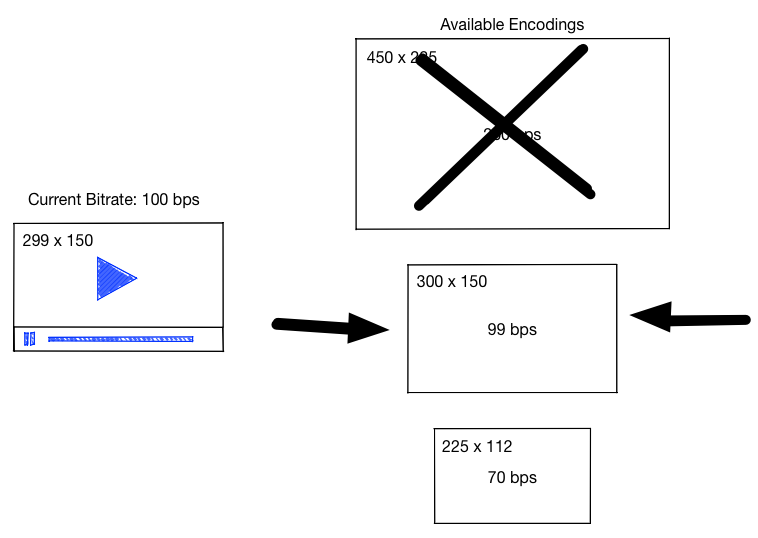
\includegraphics[width=1.0\linewidth]{images/chapter2/bitrate-switching-4.png}\hfill
 \caption[Bitrate switching]{Bitrate switching}
 \label{fig:fourV}
\end{figure}



\newpage